\documentclass{article}
\usepackage{graphicx}
\usepackage{listings}
\usepackage{ctex}
\usepackage{graphicx}
\usepackage[a4paper, body={18cm,22cm}]{geometry}
\usepackage{amsmath,amssymb,amstext,wasysym,enumerate,graphicx}
\usepackage{float,abstract,booktabs,indentfirst,amsmath}
\usepackage{array}
\usepackage{booktabs} %调整表格线与上下内容的间隔
\usepackage{multirow}
\usepackage{diagbox}
\usepackage{indentfirst}
\usepackage{bm}
\usepackage{fancyhdr}




\pagestyle{fancy}

\lhead{\bfseries \normalsize 学号:1952033\quad 姓名:侯雅玥 \quad 组员:廖宏 \\实验名称:函数产生与处理电路的实验\quad 课程名称:电子技术实验\quad 专业:微电子科学与工程 } 
\rhead{}

\begin{document}
	\section{\zihao{4} 实验名称:函数产生与处理电路的实验}
    \section{\zihao{4} 实验目的}
    \zihao {5} (1)熟悉RC桥式振荡电路和矩形波发生器的基本工作原理和电路组成形式.\par
               (2)掌握运算电路的设计与实际测量方法.\par
               (3)学会测试各运算电路的工作波形. \par
             
			   \section{\zihao{4} 实验原理}
               \subsection{正弦波发生器}
               正弦波发生器一般由自激反馈振荡器组成.有振荡频率较低的RC桥式振荡器和变压器
               反馈式振荡器,有振荡频率较高的三点式振荡器。本实验采用RC桥式振荡器           
            RC桥式振荡器如图1所示,它是由同相放大器和反馈网络两部分组成.
            RC串-并联网络组成正反馈回路,它具有选频的作用.$R_1$和$R_2$组成同相放大器负反馈回路,它们决定同相放大器放大倍数,根据反馈振荡器的振荡条件:

            \par
            幅值平衡条件
            \begin{equation*}
               \ |\dot{A}\dot{F}|=1
               \end{equation*}
               \par
               相位平衡条件
               \begin{equation*}
                \ \Phi_A+\Phi_F=2n\pi 
                \end{equation*}
                其中$\Phi_A$为放大器的相移角,$\Phi_F$为选频网络的相移角.由RC选频网络可知,
                当$\omega =\omega_0=1/RC$时,F=1/3,选频网络的相位移$\Phi_F=0$.同相放大器的$\Phi_A=0$,因而只要放大倍数略大于3,电路能产生振荡,振荡频率为
                \begin{equation*}
                    \ f_0=\frac{1}{2\pi RC}
                    \end{equation*}
                振荡幅度可调节$R_w$来实现.反馈支路中电阻并联二极管是为了达到稳幅和改善输出电压波形目的.
                \begin{equation*}
                    \ A=\frac{U_o}{U_i}=1+\frac{R_w+R_2}{R_1}
                \end{equation*}
                因此在电路中只要$|A|>3$即$R_W+R_2>2R_1$,震荡电路满足自激振荡振幅和相位起振条件
                \subsection{矩形波发生器}
                方波发生器有多种形式,图2所示的方波发生器由迟滞比较器和积分延迟环节组成.迟滞比较器方波输出,$u_{o1}$作为RC积分电路的输入,
                积分电路近似三角波输出$u_{o2}$又作为迟滞比较器的输入.电容电压$u_{o2}$上升到正向阈值电压$U_{T+}$迟滞比较器方波输出$u_{o1}$跳变为低电平$-U_Z$;电容电
                压$u_{o2}$下降到反向阈值电压$U_{T-}$迟滞比较器方波输出$u_{o1}$,跳变为高电平$+U_Z$,改变RC电路时间常数可改变矩形波频率;改变参考电压$u_R$数值或利
                用二极管单向导电性使充放电时间常数不同,可实现矩形波占空比的调节. 方波周期
                \begin{equation*}
                    \ T=RCln\frac{U_Z-U_{T-}}{U_Z-U_{T+}}\times \frac{U_Z+U_{T+}}{U_Z+U_{T-}}
                \end{equation*}


   

\section{\zihao{4} 实验电路}
\begin{figure}[h]
	\begin{minipage}[t]{0.5\linewidth} % 如果一行放2个图,用0.5,如果3个图,用0.33  
	  \centering   
	  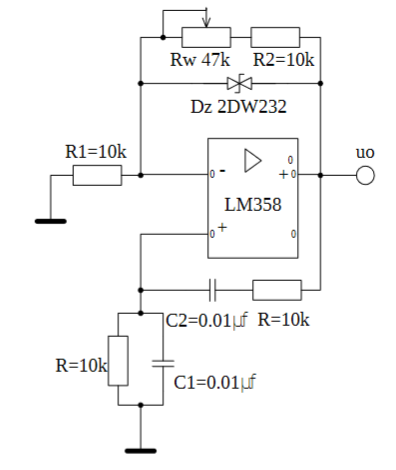
\includegraphics[width=3in]{H:/电子技术试验/4-16/4-16-1.png}   
	  \caption{RC桥式振荡器}   
	  \label{fig:side:a}   
	\end{minipage}%   
	\begin{minipage}[t]{0.5\linewidth}   
	  \centering   
	  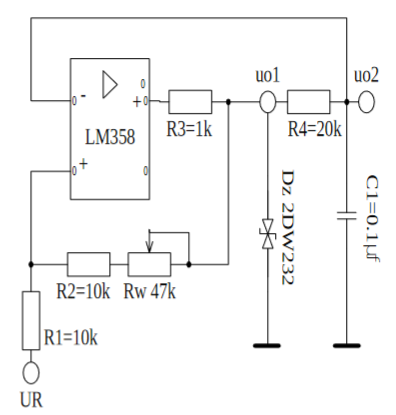
\includegraphics[width=3in]{H:/电子技术试验/4-16/4-16-2.png}   
	  \caption{方波发生器}   
	  \label{fig:side:b}   
	\end{minipage}   
  \end{figure}


\section{\zihao{4} 实验内容及步骤}
  \subsection{RC桥式振荡电路}
(1)按图1接线,检查后通电。调节电位器Rw,在输出端得到稳定的基本不失真的正弦波。\par
(2)用示波器观察和记录输出波形的幅度、频率。最后记录Rw的实际阻值。

 \subsection{方波发生器}
 (1)按图2接线,检查后通电。
 (2)先使$U_R=0(V)$,调节电位器Rw使Uo1的频率f=500Hz,用示波器记录Uo1、Uo2的图像。
 (3)保持Rw不变,按表1要求完成实验。

 
\newpage


\section{\zihao{4} 数据及误差处理}
\subsection{RC桥式震荡电路}

\begin{figure}[h]
    %\small
    \centering
    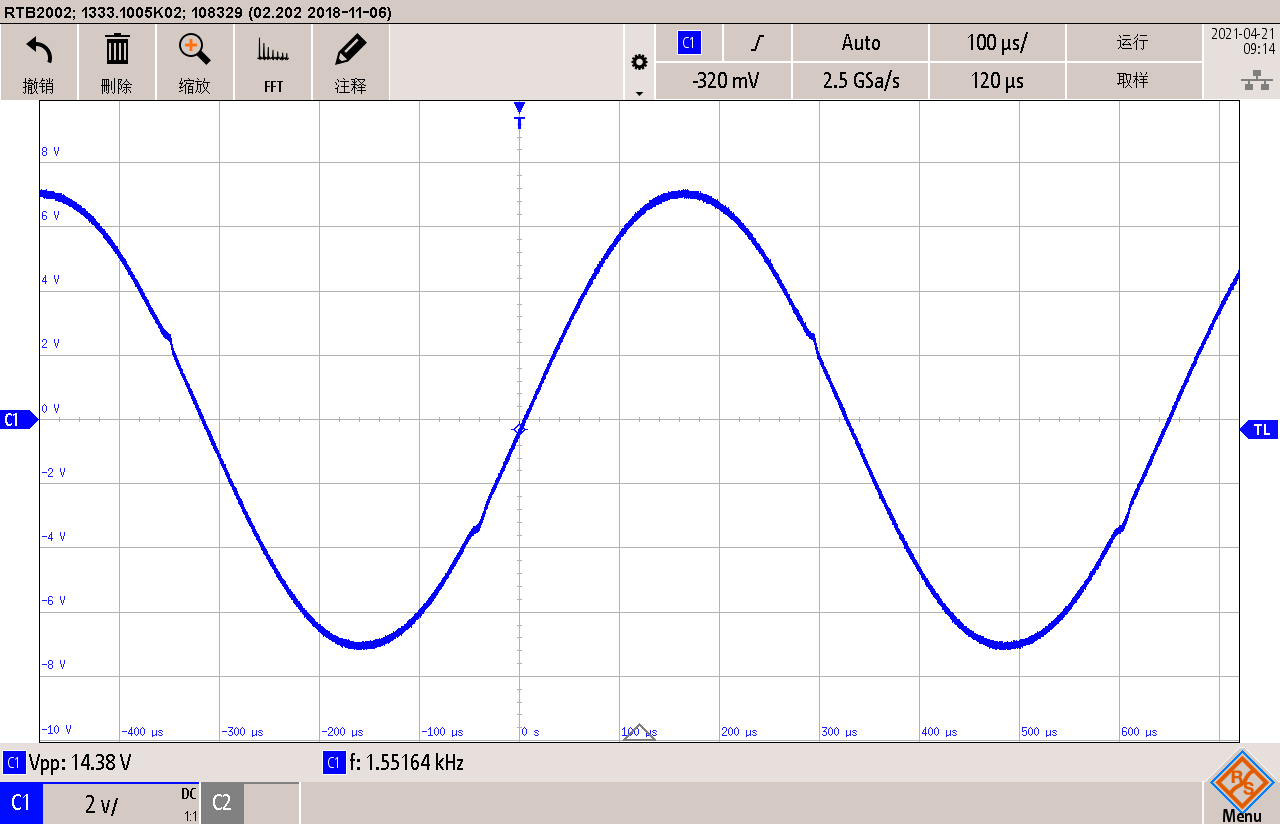
\includegraphics[width=3in]{H:/电子技术试验/4-16/4-16-3.png}
    \caption{产生的稳定正弦波} \label{fig:aa}
\end{figure}
产生的正弦波的:\par
幅度测量值:\[A_m=7.22V\]\par
频率测量值:\[f=1.55kHz\]\par
测得测量值:\[R_w=10.37k\Omega\]\par
电压增益:
\begin{equation*}
    \ A_u=\frac{U_o}{U_i}=1+\frac{R_w+R_2}{R_1}=3.04
\end{equation*}\par
满足自激振荡的振幅和相位起振条件\par
频率理论值:\[f_0=\frac{1}{2\pi RC}=1.59kHz\] \par
频率相对误差:\[\delta (f)=\frac{f_0-f}{f_0}=2.52\%\]\par
\newpage

\subsection{方波发生器}
\begin{table}[h]
    \centering  
    \begin{tabular}{c|c|c|c}
        \hline
            $U_{R}(V)$      & f(Hz)         & 正占空比($\%$)    & $U_{o1},U_{o2}$图像 \\ \hline
              0             & 499.97       &  48.40\%           &  $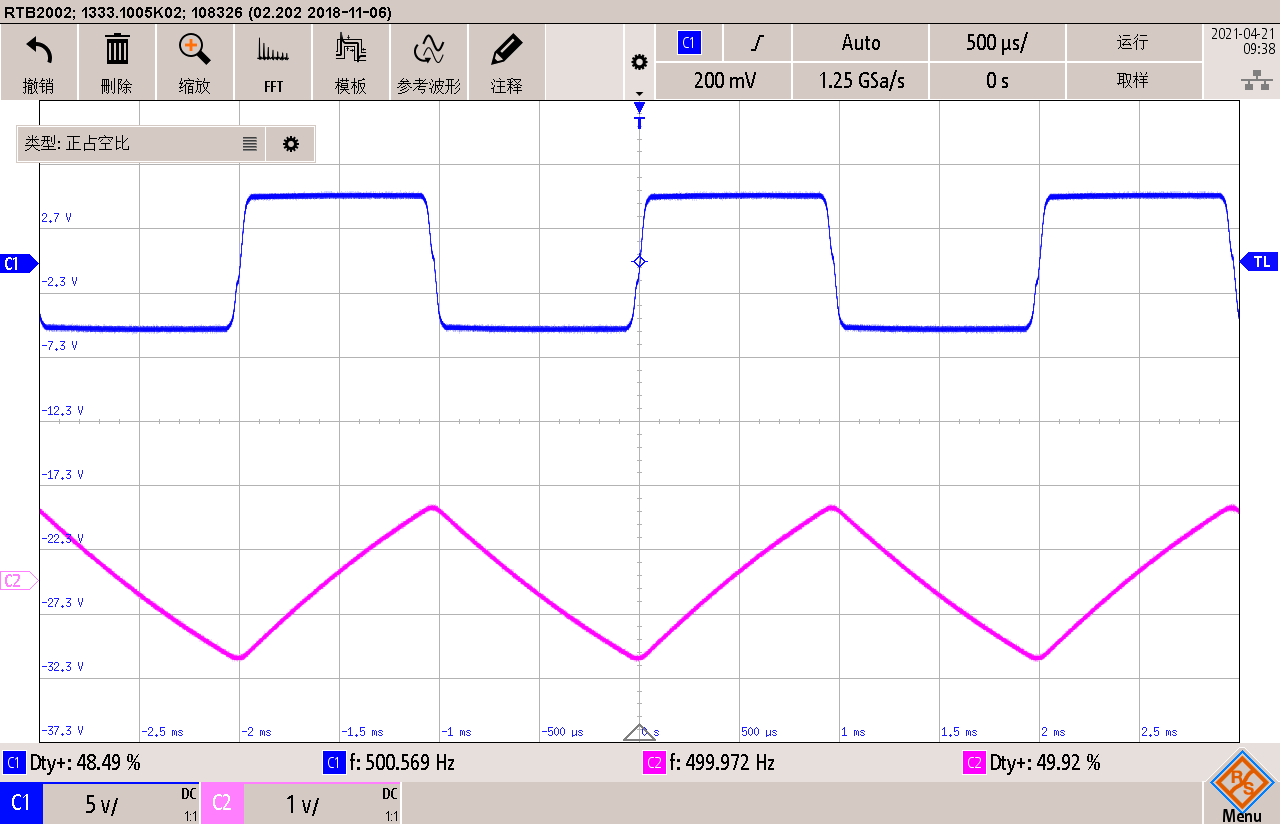
\includegraphics[width=1.9in]{H:/电子技术试验/4-16/4-16-6.png}$  \\ \hline
              1             & 477.56       &  56.35\%           &  $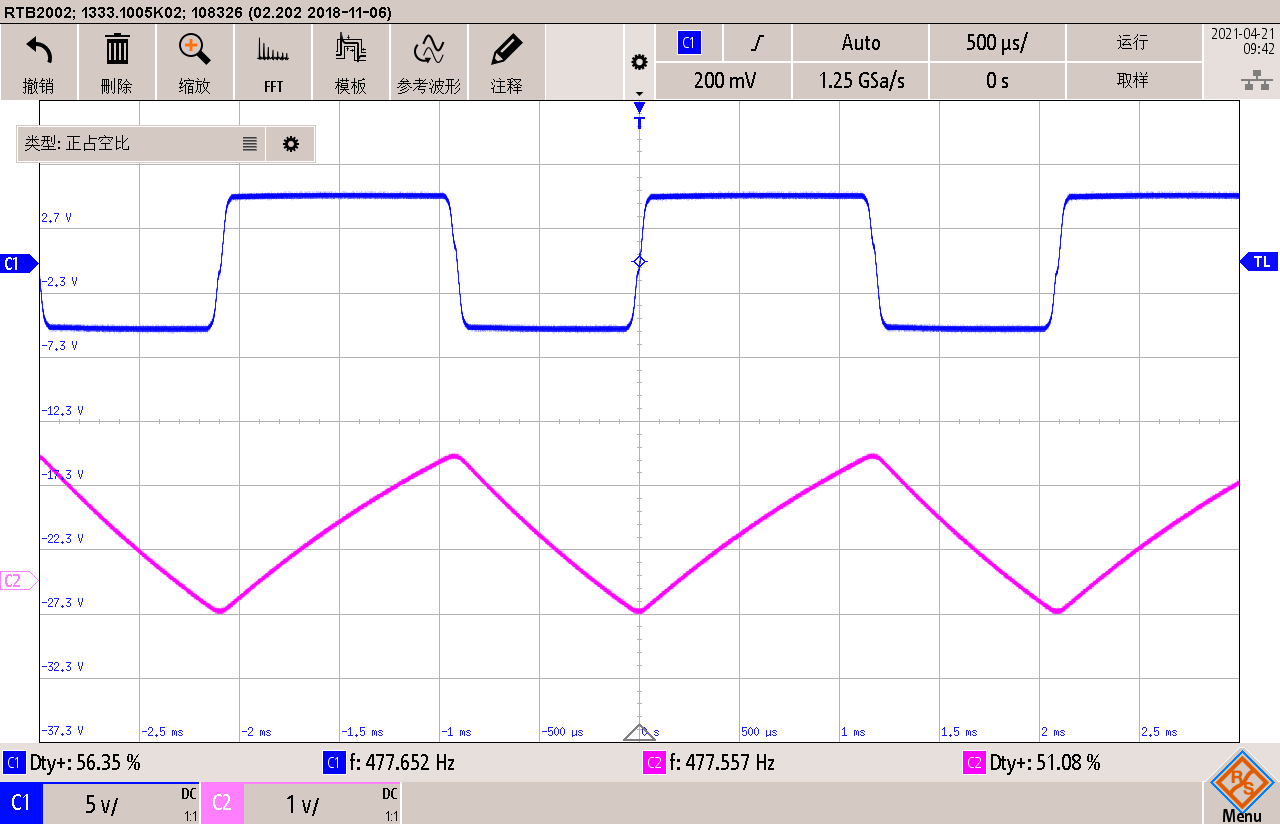
\includegraphics[width=1.9in]{H:/电子技术试验/4-16/4-16-5.png}$             \\ \hline
              2             & 439.70       &  64.20\%           &  $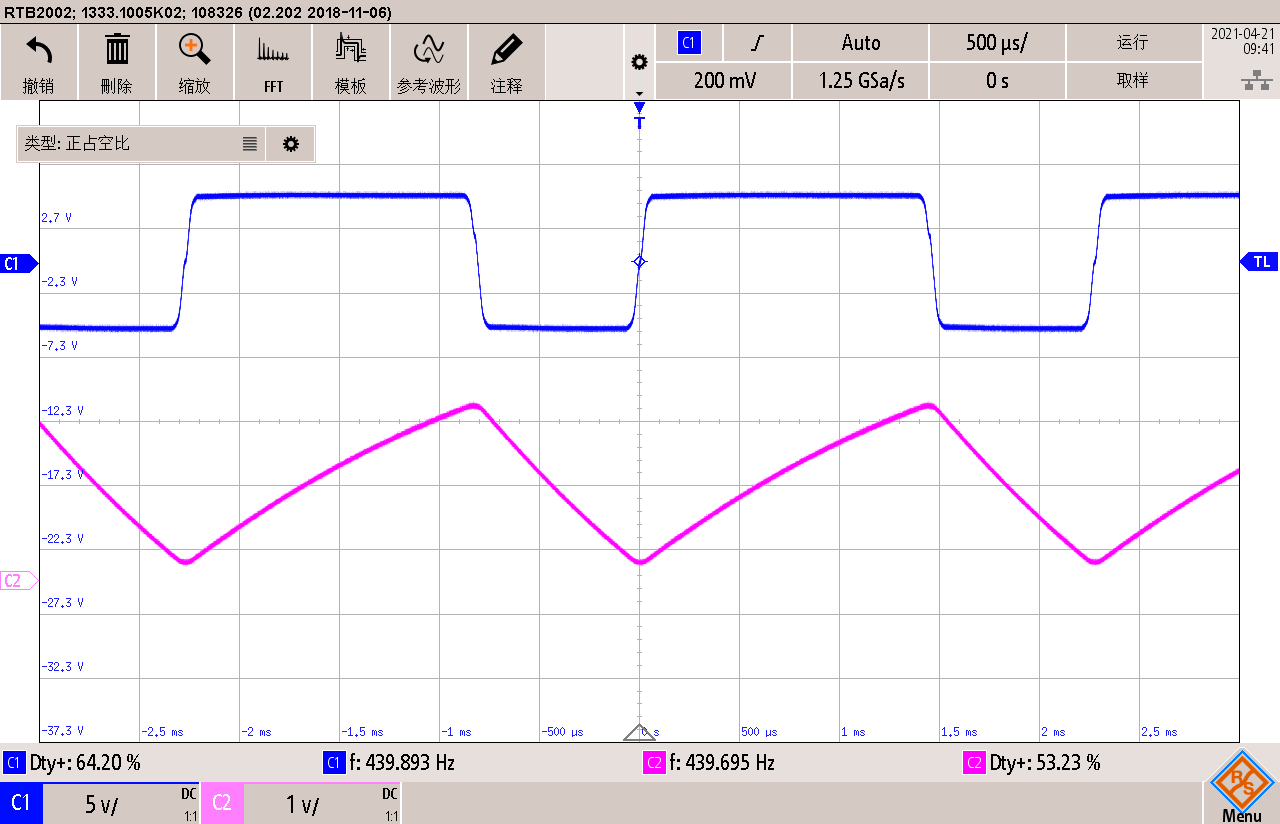
\includegraphics[width=1.9in]{H:/电子技术试验/4-16/4-16-4.png}$           \\ \hline
              -1            & 482.549      &  40.47\%           &  $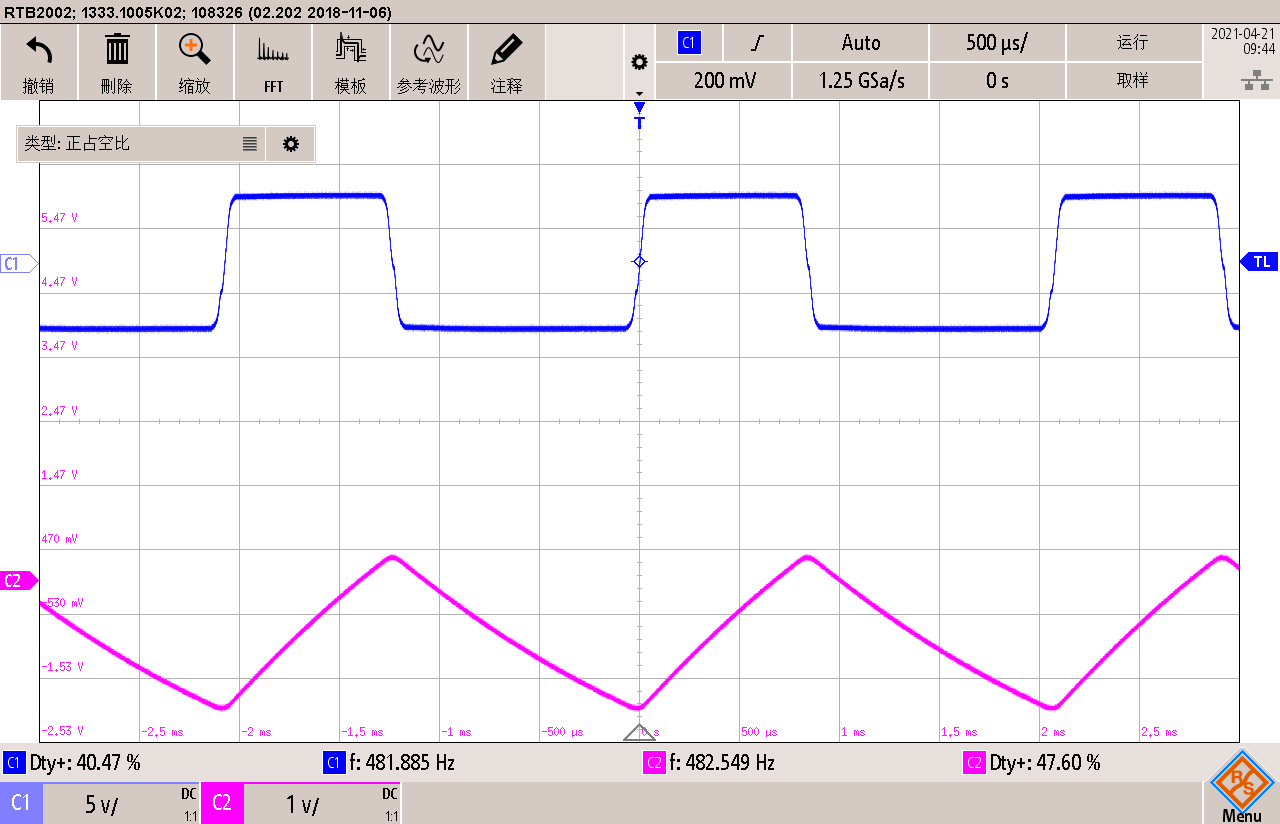
\includegraphics[width=1.9in]{H:/电子技术试验/4-16/4-16-7.png}$          \\ \hline
              -2            & 446.13       &  32.47\%           &  $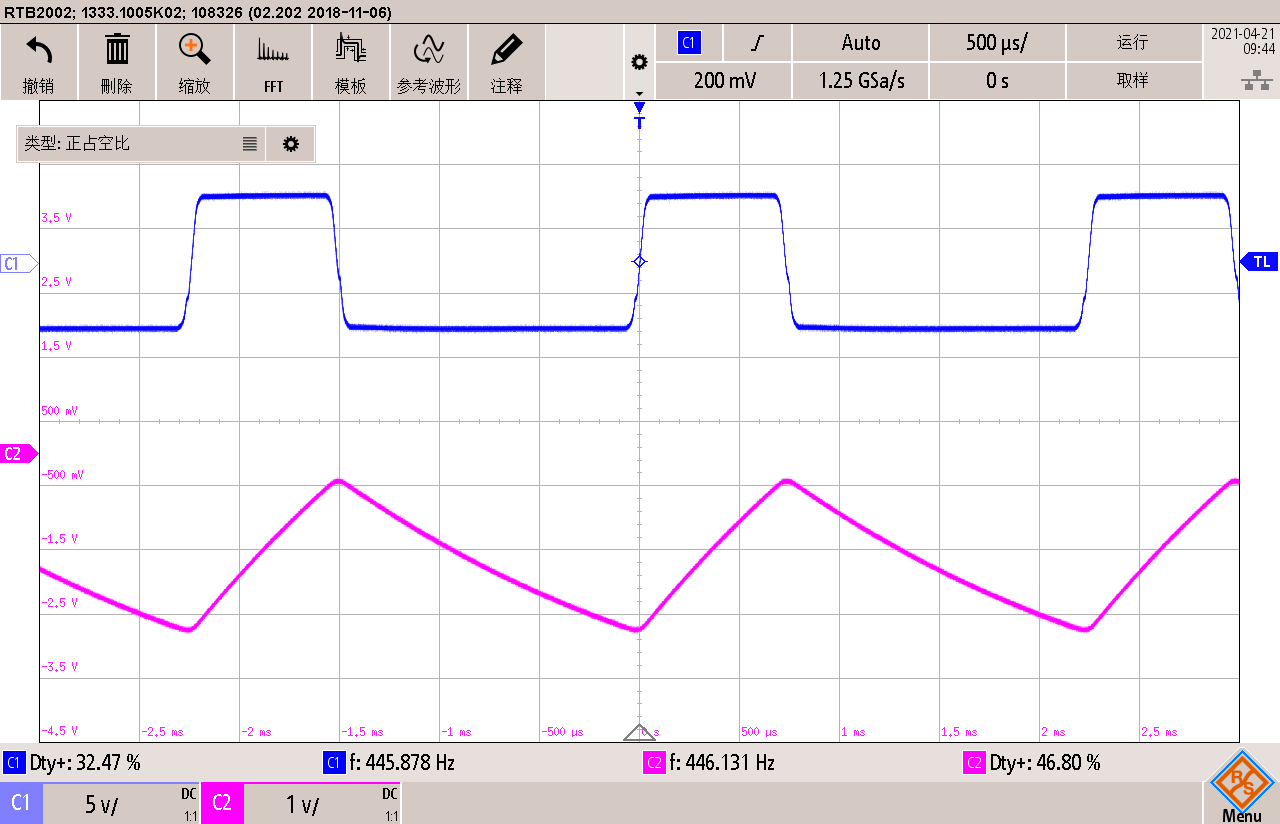
\includegraphics[width=1.9in]{H:/电子技术试验/4-16/4-16-8.png}$        \\ \hline
    \end{tabular}
  \end{table}
\newpage
由
\begin{equation*}
  \ T=RCln\frac{U_Z-U_{T-}}{U_Z-U_{T+}}\times \frac{U_Z+U_{T+}}{U_Z+U_{T-}}
\end{equation*}
得到
\begin{table}[h]
  \centering  
  \begin{tabular}{c|c|c|c}
      \hline
          $U_{R}(V)$      & f(Hz)         & $f$理论值   & $\delta (f) $\\ \hline
            0             & 499.97       &  500.92           &  0.19\% \\ \hline
            1             & 477.56       &  482.63           &  1.05\%           \\ \hline
            2             & 439.70       &  440.68           &  0.22\%        \\ \hline
            -1            & 482.55      &  483.01            &  0.09\%  \\ \hline
            -2            & 446.13       &  452.23           &  1.34\%    \\ \hline
  \end{tabular}
\end{table}

	\section{\zihao{4} 实验设备和器材}
	(1)双踪示波器             \qquad \qquad \qquad \qquad \qquad  \qquad           1台\par
	(2)直流稳压电源             \qquad \quad \qquad \qquad \qquad \qquad           1台\par
	(3)模拟电路实验箱            \qquad  \qquad \qquad \qquad\qquad                1台\par
	(4)万用表                   \qquad  \qquad \qquad \qquad \qquad \qquad \qquad  1只\par
	(5)集成芯片LM358、电阻器、电容器  \quad                                        若干

\section{结论}
\subsection{RC桥式振荡电路}
(1)起振过程\par
电路中存在各种电扰动,经过选频网络通过反馈产生比较大的反馈电压。通过线性放大和反馈的不停循环,振荡电压就会不断增大。
(2)振荡频率\par
振荡频率由相位平衡条件决定。
,仅在\begin{equation*}
  \ |\dot{A}\dot{F}|=1
  \end{equation*}
处满足相位平衡条件,所以振荡频率为:
 \begin{equation*}
  \ f_0=\frac{1}{2\pi RC}
  \end{equation*}
改变R、C可改变振荡频率

\subsection{矩形波发生器}
方波发生器由迟滞比较器和积分延迟环节组成改变RC电路时间常数可改变矩形波频率;改变参考电压$u_R$数值或利
用二极管单向导电性使充放电时间常数不同,可实现矩形波占空比的调节. 方波周期
\begin{equation*}
    \ T=RCln\frac{U_Z-U_{T-}}{U_Z-U_{T+}}\times \frac{U_Z+U_{T+}}{U_Z+U_{T-}}
\end{equation*}
\section{思考}
(1)当运算理想时,输出电压的幅值将是无穷大,但是由于运方式上有一个最大输出电压,所以输出电压的幅值实际上由运放的最大输出电压控制,无法由电路的参数求出\par
(2)振荡幅度的增长过程不可能永无止境的延续下去,当放大器逐渐由放大区进入饱和区或截止区。工作于非线性状态,其增益逐渐下降,当放大器增益下降导致环路增益下降为1,振幅增长过程将停止,振荡器达到平衡。\par
(3)由运放构成的RC串并联正弦波振荡电路不是靠运放内部的晶体管进入非线性区稳幅,而是通过在外部引入负反馈来达到稳幅的目的。 \par

\end{document}